\section{Theoretical Analysis}
\label{sec:analysis}

In this section, the circuit shown in Figure~\ref{fig:Cir} is analysed
theoretically, to determine all mesh currents and nodes voltages.
In Figure~\ref{fig:Cir_teo}, conventions that will be used doing mesh and nodes analysis are shown.

\begin{figure}[h] \centering
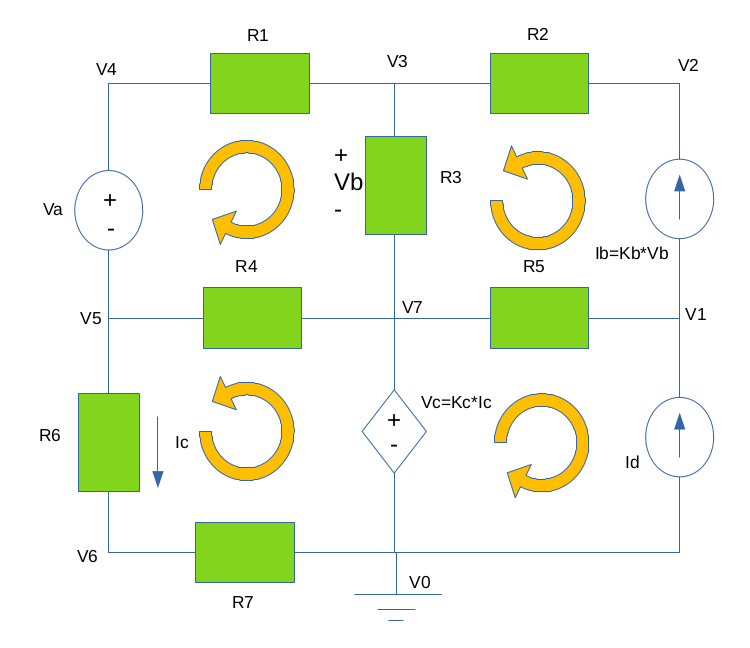
\includegraphics[width=0.8\linewidth]{Esquema_teor.png}
\caption{Circuit with nodes and currents convention}
\label{fig:Cir_teo}
\end{figure}

\section{Mesh analysis}

By inspection, the circuit has four meshes, in each one, the current flows like in Figure~\ref{fig:Cir_teo}. Since there is four variables, $I_1$, $I_2$, $I_3$ and $I_4$, we'll need four linearly independent equations, to get them we'll apply KVL to mech '1' and mesh '3' since they don't have current sources that hinder the job, the twor equations will be,

\begin{equation}
  Va = R1 \dot I_1+R3(I_1 + I_2) + R4(I_1 + I_3)
  \label{eq:KVL1}
\end{equation}

\begin{equation}
  Vc = R4(I_3 + I_1) + R6 \dot I_3 + R7 \dot I_3
  \label{eq:KVL3}
\end{equation}

we can see now, that in equation~\ref{eq:KVL3}, we added a new variable, $Vc$, so we'll need to find another equation and since we know by inspection that $Ic=I_3$, we can easily get,

\begin{equation}
  Vc = Kc \dot I_3.
  \label{eq:Vc}
\end{equation}

Now we still need two other equations, we find one by analysing the dependente current source, the voltage drop in $R3$ and detecting that $I_2=Ib$,

 \begin{equation}
  \frac{I_b}{Kb} = Vb = (I_1 + I_2)R3  \frac{I_2}{Kb} = (I_1 + I_2)R3.
  \label{eq:Vb}
\end{equation}

Again by inspection we get $I_4 = -Id$ which finalises our equations.
To resolve this equations we put them in matrix form and we then used octave to resolve the matrix equation a lot easier.

The theoretical values were COMPLETAR!!!!

\section{Node analysis}

For the node analysis we number the nodes as in Figure~\ref{fig:Cir_teo}, as said. For this method we'll work with conductance instead of resistors because it makes it easier to work with. We now have eight variables so we'll have to find eight equations. Since we defined ground in node zero we get the first equation, which is $V_0=0$. The next four equations we get from doing KCL in nodes 1, 2 3 and 6 since they don't have voltage sources, which makes it easier. The equations are the following,
Node 1:

 \begin{equation}
  -Id + Ib - G5(V_7-V_1) = 0.
  \label{eq:N1}
\end{equation}

Node 2:

 \begin{equation}
  -Ib + G2(V_2-V_3) = 0.
  \label{eq:N2}
\end{equation}

Node 3:

 \begin{equation}
  -G2(V_2-V_3)-G1(V_4-V_3)-G3(V_3-V_7) = 0.
  \label{eq:N3}
\end{equation}

Node 6:

 \begin{equation}
  G7(V_6-V_0)-G6(V_5-V_6) = 0.
  \label{eq:N6}
\end{equation}

From this equations we see that we added a new unknown variable, $Ib$, for that reason we need to add another equation, we'll use the current source and the voltage drop in $R3$, knowing that,

 \begin{equation}
  I_b = Kb \dot Vb = Kb(V_3-V_7) Ib = Kb(V_3-V_7).
  \label{eq:Ib}
\end{equation}

We still need three equations. We'll get one from de voltage drop in $Va$ and from the voltage drop in the dependent voltage source. This two equations are,

  \begin{equation}
  V_4-V_5 = Va
  \label{eq:Va}
\end{equation}

and

 \begin{equation}
  V_7-V_0 = Kc \dot Ic = Kc\dot G6(V_5-V_6) V_7-V_0 = Kc\dot G6(V_5-V_6).
  \label{eq:Vc}
\end{equation}

The final equation equation will be from the the node seven but since we don't easily know the current that flows through the dependent current source, we first need to find a equation for this current, for that we'll analyse node 0 and doing that we get the equation

 \begin{equation}
  I = G7(V_6-V_0) - Id
  \label{eq:corrente}
\end{equation}

, where $I$ is the current we are trying to find. Now doing the node analysis for node 7 we get the equation,

 \begin{equation}
  G5(V_7-V_1)+G4(V_7-V_5)-G3(V_3-V_7)-G7(V_6-V_0)+Id = 0.
  \label{eq:N3}
\end{equation}

We finaly have a sistem of linearly equations that we can resolve using matrix form in octave.
The theoretical values are COMPLETAR!!!!!!!!!!!!!
